\subsection{Tipo de entidad Plantilla Entrevista Asesor}

   \begin{description}

   \item[Definición] Se refiere al objeto del mundo real: \emph{``Conjunto de
   preguntas que realiza un asesor en un momento determinado, de forma
   individual o grupal a los alumnos, que él mismo se crea''}.

   \item[Características] La entidad presenta las siguientes características:
      \begin{itemize}
         \item \textbf{Nombre:} Plantilla Entrevista Asesor.
         \item \textbf{Tipo:} Fuerte.
         \item \textbf{Número de atributos:} 1 propio y 2 heredados.
         \item \textbf{Atributo/s identificador/es principal/es:} id\_entrevista\_asesor.
         \item \textbf{Atributo/s identificador/es alternativo/s:} -
         \item \textbf{Atributo/s heredado/s:} dni\_pasaporte y curso\_académico
         del tipo de entidad Asesor Curso Académico.
      \end{itemize}

   \item[Diagrama] La figura \ref{diagramaPlantEntAse} muestra el diagrama de la entidad.
   \item \begin{figure}[!ht]
            \begin{center}
            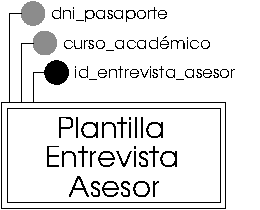
\includegraphics[]{07.Modelo_Entidad-Interrelacion/7.2.Analisis_Entidades/diagramas/plant_ent_ase.pdf}
            \caption{Diagrama de la entidad Plantilla Entrevista Asesor.}
            \label{diagramaPlantEntAse}
            \end{center}
         \end{figure}

   \item[Descripción de los atributos propios] Esta entidad presenta el
   siguiente atributo propio:

   \begin{itemize}
    \item \textbf{id\_entrevista\_asesor}
      \begin{itemize}
         \item \textbf{Definición:} Código que sirve como número identificativo
               para cada plantilla de entrevista de asesor del sistema.
         \item \textbf{Dominio:} Números naturales.
         \item \textbf{Carácter:} Obligatorio.
         \item \textbf{Ejemplo práctico:} 36.
         \item \textbf{Información adicional:} El dato lo genera el sistema
               cuando se introduce una nueva plantilla de entrevista de asesor
               en el sistema. Es la clave primaria.
      \end{itemize}
   \end{itemize}

   \item[Ejemplo práctico]

   \item \begin{center}
            \begin{tabular}{ | l | l | }
            \hline
            \multicolumn{2}{ | c | }{\textbf{Tipo de entidad Plantilla Entrevista Asesor}} \\
            \hline
            dni\_pasaporte & 98765432Z \\
            \hline
            curso\_académico & 2008 \\
            \hline
            id\_entrevista\_asesor & 36 \\
            \hline
            \end{tabular}
         \end{center}
   \end{description}
